\documentclass[11pt,parskip=full,a4paper,titlepage,oneside,bibliography=totocnumbered]{scrreprt}
\usepackage[utf8]{inputenc}
\usepackage[english]{babel}
\usepackage{amsmath}
\usepackage{amsfonts}
\usepackage{amssymb}
\usepackage{siunitx}
\usepackage{xcolor}
\usepackage{graphicx}
\usepackage{scrpage2}
\usepackage[left=2cm,right=2cm,top=2cm,bottom=3cm]{geometry}
\usepackage{listings}
\usepackage{textcomp}
\usepackage{wrapfig}
\usepackage{subfigure}
\usepackage{caption}
\usepackage{float}
\usepackage{tabularx}

\usepackage{enumitem}

\usepackage{helvet}
\usepackage{charter}
%\usepackage{lmodern}

\lstset{belowcaptionskip=1\baselineskip,
  breaklines=true,
  frame=L,
  xleftmargin=\parindent,
  showstringspaces=false,
  basicstyle=\footnotesize\ttfamily\color{gray},
  escapeinside={(*@}{@*)},}

\lstdefinestyle{customc}{
	belowcaptionskip=0\baselineskip,
	breaklines=true,
	frame=L,
	xleftmargin=\parindent,
	language=C,
	showstringspaces=false,
	basicstyle=\footnotesize\ttfamily,
	keywordstyle=\bfseries\color{green!40!black},
	commentstyle=\itshape\color{purple!40!black},
	identifierstyle=\color{blue},
	stringstyle=\color{orange},
}


\renewcommand*{\chapterformat}



\author{Julian Daberkow}
\title{PLATZHALTER - TITEL}

\date{\today}

\begin{document}
\begin{titlepage}

\begin{center}


% Oberer Teil der Titelseite:
\includegraphics[width=0.20\textwidth]{./media/QUT_Square_black.jpg}\\[1cm]    

\textsc{\LARGE ENB350: Real-Time Computer-Based Systems}\\[1.5cm]

\textsc{\Large Semester 1 2016}\\[0.5cm]


% Title
\newcommand{\HRule}{\rule{\linewidth}{0.5mm}}
\HRule \\[0.6cm]
{ \huge \bfseries Problem Based Learning Assignment}\\[0.4cm]

\HRule \\[1.5cm]

% Author and supervisor
\begin{minipage}{0.4\textwidth}
\begin{flushleft} \large
\emph{Authors:}\\
Julian \textsc{Daberkow} (9637516)\\
Timo \textsc{Michalski} (9637532)\\
Hendrik \textsc{Oestreich} (9637508)
\end{flushleft}
\end{minipage}
\hfill
\begin{minipage}{0.4\textwidth}
\begin{flushright} \large
\emph{Lecturer:} \\
Prof. Vinod \textsc{Chandran}\\
\hfill\\
\hfill\\
\hfill\\
\end{flushright}
\end{minipage}

\vfill

% Unterer Teil der Seite
{\large \today}

\end{center}

\end{titlepage}

\tableofcontents
\listoffigures
\listoftables
\chapter{Introduction} \label{ch:Introduction} % (2 pages)

\section{Problem Statement} \label{sec:ProblemStatement}
In a production line, different work pieces have be checked in the beginning to make sure only work pieces which meet all requirements are further processed. Therefore a MPS testing station of the vendor Festo is used, which provides a set of sensors and work piece handling components / actuators (see Fig.\ref{fig:festostation}). The sensors and actuators of the station are connected to the GPIO Pins of the micro-controller of the \textit{Tiva Development Kit DK-TM4C129X}. This allows controlling the actuators (activation or deactivation) and reading sensor values.

\begin{figure}[H]
	\begin{center}
		\includegraphics[scale=.50]{media/FestoStation.png} 	
		\caption{Festo Station}
		\label{fig:festostation}
	\end{center}
\end{figure}

The testing process is structured into the following steps:
\begin{enumerate}[noitemsep]
	\item Workpiece is placed onto a platform.
	\item Color and material is sensed with the related sensors in this position(see Fig. \ref{fig:festostationsensorsandejector} and Fig.\ref{fig:festostationcolorandmaterialsensor}).
	\item A safety light barrier is used to ensure that the hands of the operator of the station are not in the zone of the moving parts any more.
	\item The platform is moved up (see Fig.\ref{fig:festostationliftingmodule}).
	\item In the top position a height measurement is triggered (see Fig.\ref{fig:festostationheightmeasurement}).
	\item Based on the height measurement a work piece is accepted within certain thresholds or rejected if beyond.
	\item If the work piece is accepted the following steps are executed:
	\begin{enumerate}
		\item The ejector which is attached to the platform pushes the work piece onto a pneumatic slide (see Fig.\ref{fig:festostationsensorsandejector}). 
		\item The pneumatic slide is activated to transfer the work piece to the next station in the production process (see Fig.\ref{fig:festostationpneumaticslide}).
		\item The ejector is retracted.
		\item The platform is moved down.
	\end{enumerate} 
	\item If it is rejected the following steps are executed:
	\begin{enumerate}
		\item The platform is moved down.
		\item The ejector which is attached to the platform pushes the work piece onto a  slide which is not further automated.
		\item The ejector is retracted.
	\end{enumerate}
\end{enumerate}


\begin{figure} [H] 	
	\begin{center}
		\subfigure[Festo Station Height Measurement]{\includegraphics[width=0.4\textwidth]{media/FestoStation_HeighMeasurement.png}
			\label{fig:festostationheightmeasurement}} 
		\hspace{0.05\textwidth}
		\subfigure[Festo Station Senors and Ejector]{\includegraphics[width=0.4\textwidth]{media/FestoStation_SensorsAndEjector.png}
			\label{fig:festostationsensorsandejector}} 
		\caption{Festo Station Detail}
		\label{fig:festostationdetail}
	\end{center}
\end{figure} 

\begin{figure} [H] 	
	\begin{center}
		\subfigure[Festo Color and Material Sensor]{\includegraphics[width=0.25\textwidth]{media/FestoStation_ColorAndMaterialSensor.png}
			\label{fig:festostationcolorandmaterialsensor}} 
		\hspace{0.05\textwidth}
		\subfigure[Festo Lifting Module]{\includegraphics[width=0.25\textwidth]{media/FestoStation_LiftingModule.png}
			\label{fig:festostationliftingmodule}} 
		\hspace{0.05\textwidth}
		\subfigure[Festo Pneumatic Slide]{\includegraphics[width=0.25\textwidth]{media/FestoStation_PneumaticSlide.png}
			\label{fig:festostationpneumaticslide}} 
		\caption{Festo Modules Detail}
		\label{fig:festomodulesdetail}
	\end{center}
\end{figure} 

\section{Requirements}
The task was to fully automate the testing process by implementing a test program which runs on the micro-controller and operates based on the sensor values as an input and controls the actuators in a real time manner. The Task was spilt up into two sections:
Firstly a device driver should be written to allow a high level access to the GPIO ports, encapsulated in meaningful methods. The device driver should provide methods for each of the tasks (and subtasks) mentioned in section \ref{sec:ProblemStatement}. A special requirement was also the conversion of the analogue height measurement signal to a meaningful digital value.
Secondly an application program should be written which controls the execution of the testing process, allows the user to start, stop and configure it and display relevant information on the touch screen of the Tiva development board. This included methods for the calibration of the height measurement, the setting of threshold values and keeping track of all processed work pieces. Additionally the calendar time should be displayed and a throughput should be calculated.

\section{Contributions}
The display logic and the interaction with the main program was developed by Julian Daberkow. The device driver was developed by Timo Michalski and Hendrik Oestreich and integrated into the main program. They also developed the state machine which controls the execution of the testing process. The overall integration of all components including the communication between the different tasks was done by Julian Daberkow and Timo Michalski. 






\chapter{Design and Implementation}

(approx. 10 pages)\\
* Approach to design\\
* important issues and choices and their relationships to theoretical concepts and the hardware and software platforms\\
* You can use one subsection for the driver and another for the data logger.\\

* Check if you have addressed Provided a graphical representation for your design?\\
* Provided a Project folders and files diagram?\\
* Did you use the GPIO module? How?\\
* Did you use the graphics library? How?\\
* Did you use interrupts? How?\\
* Did you use multiple threads / handlers? How? Why?\\
* Did you use the ADC? How? Did you use TI-RTOS? How?



\begin{figure}[H]
	\begin{center}
		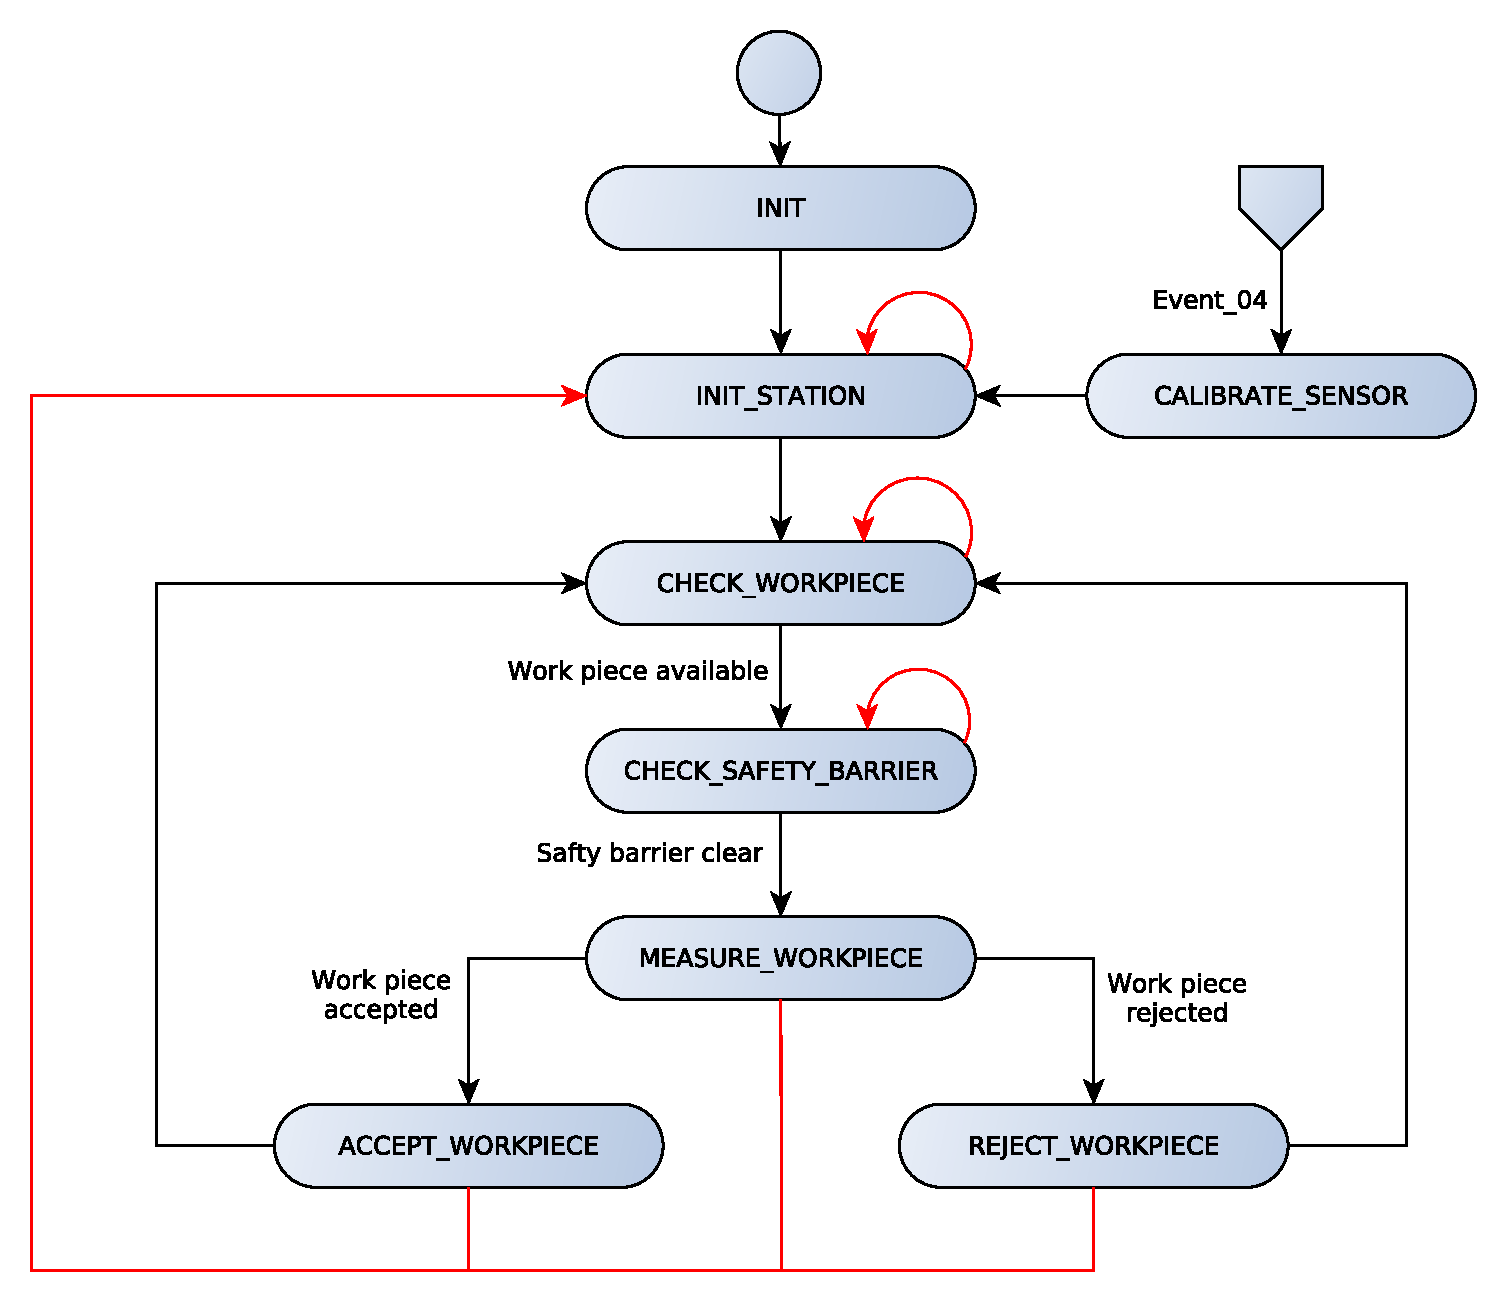
\includegraphics[scale=.50]{media/StateMachine_Main.png} 	
		\caption{Main State Machine}
		\label{fig:statemachine}
	\end{center}
\end{figure}



\begin{figure}[H]
	\begin{center}
		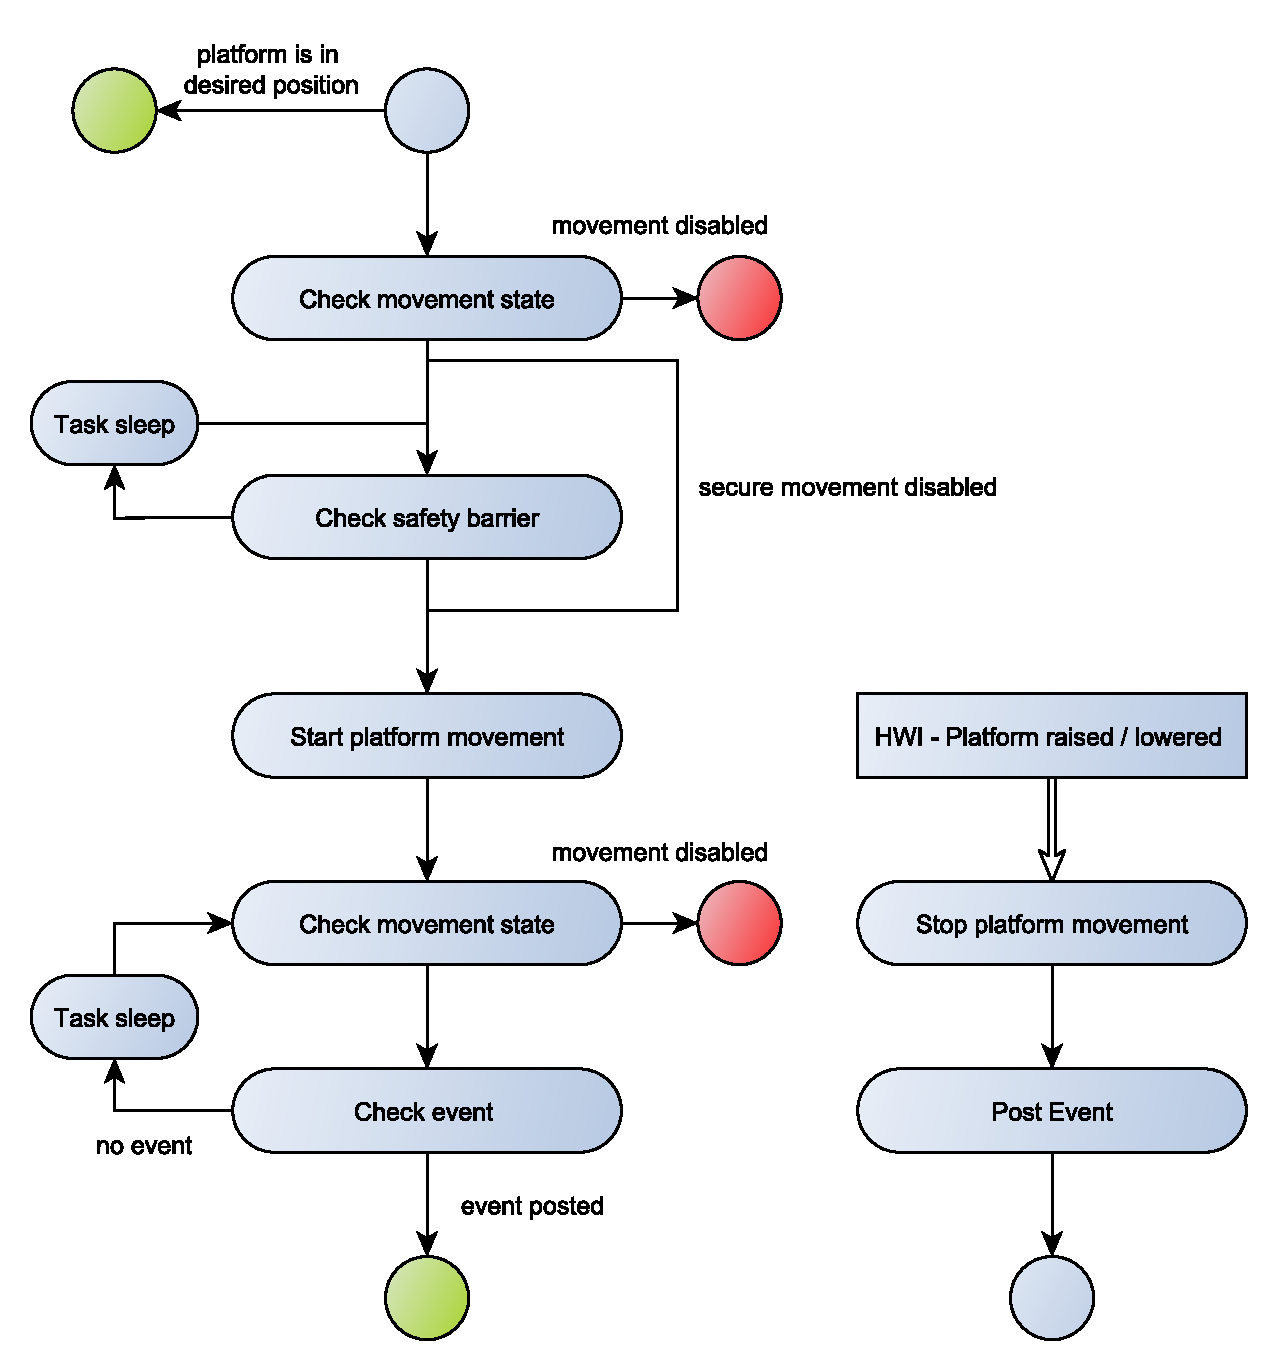
\includegraphics[scale=.40]{media/Flow_Chart_MovePlatform.png} 	
		\caption{Flow Chart Move Platform}
		\label{fig:moveplatform}
	\end{center}
\end{figure}
\chapter{Results} \label{ch:results}%(2 pages)\\

The project was successfully realised and all functional requirements were implemented and are working during operation:

\begin{list}{\makebox[0pt][l]{$\square$}\raisebox{.15ex}{\hspace{0.1em}$\checkmark$}}
	\item The station works in a fully automated mode to test the inserted work pieces and accepts or rejects them based on their height measurements.
	\item %dirty hack, but somehow it does not work without
	\item The testing process can be started or stopped by the hardware buttons on the development board.
	\item The screen in the development board displays all required information for the current work piece and an overview over the whole test period.
	\item The application also allows the operator to use a calibration procedure in which he will be guided by the user interface.
	\item The thresholds for accepted work pieces can be adjusted in the user interface.
	\item The LED on the development board shows the current status or the station (active = green / stopped = red).
	\item The current calendar time is displayed and updated periodically.
	\item The automation process calls all functions from the self-developed device driver library and does not call any lower level functions for pin access.
\end{list}

In hindsight a few things could have been implemented differently to have a better code quality and more consistency overall. For example sometimes boolean variables are used in the code and at other places the same behaviour is implemented based on an event polling mechanism. 

Currently only the hardware interrupt of the platform sensors (up and down position) are causing a direct reaction in the program. The same handling might as well be implemented for the hardware button which starts or stops the station. In case the stopping is seen as an emergency stop, the reaction should be as a real-time requirement and not only if the related task is scheduled the next time. 

For a better user experience in operating the station the graphical interface can be advanced and it may be evaluated if touch screen interactions are preferred by users instead of the handling with the hardware buttons. Another thing that should be advanced is the flickering of the LCD which is due to the clearing of the entire screen when updating the informations on it. Double buffering techniques could be used like mentioned in section 3.1 of \cite{Wilson:2013}.

During operations we noticed that the safety barrier does not provide enough safety for the operator. The problem is that is has to be ignored as soon as the platform should move up, since during movement it also activates the safety barrier and would stop the movement which is not wanted. As a solution a delay can be inserted after a work piece is sensed and the platform is only moved after the time of the delay has passed. On the other hand this would decrease the possible throughput which would be a negative aspect if one would think of using the testing station for real-world scenarios in industry.


\appendix
\begin{thebibliography}{9}

\bibitem[TI-RTOS]{TI-RTOS}
TI-RTOS 2.10 - User's Guide, Texas Instruments, November 2014.

\bibitem[SYS/BIOS]{SYS/BIOS}
SYS/BIOS (TI-RTOS Kernel) v6.45 - User's Guide, Texas Instruments, December 2015.

\bibitem[Tiva Graphics]{TiveGraphics}
TivaWareTM Graphics Library - User's Guide, Texas Instruments, February 2014.

\bibitem[Wilson13]{Wilson:2013}
Wilson, D. (2007). TivaWareTM Graphics Library Display Drivers - Application Report. Texas 
Instruments, July 2013.

\bibitem[Festo]{Festo}
Festo Didactic Catalogue (2014), Festo Didactic GmbH \& Co. KG, pp. 290-291, 2013.
 
\end{thebibliography}

\begin{table}[H]
	\begin{tabu} spread \linewidth {l | l | X[m]}
		\textbf{Document} & \textbf{Report (Sub-)Section} & \textbf{Keyword} \\
		\hline
		\hline
		TI-RTOS & - & -\\
		\hline
		SYS/BIOS & \ref{ch:designAndImplementation} & Hardware Interrupts, Software Interrupts, Tasks, Events\\
		\hline
		Tiva Graphics & \ref{sec:ui} & \texttt{GrStringDraw}, \texttt{GrRectDraw}\\
		\hline
		Wilson13 & \ref{ch:results} & Double buffering, Off-Screen Display Drivers\\	
	\end{tabu}
	\caption{Bibliography Links}
	\label{tab:BibliographyLinks}
\end{table}

%\vfill
\chapter{Appendix}

(1 page)\\
* Mention the name of the hardware development platform and versions of the tools used such as Code Composer Studio, Tivaware, RTOS etc.

\begin{table}[H]
	\begin{tabularx}{\textwidth}{l | X}
		Platform / Tool & Version \\
		\hline
		Development Kit & TivaTM C Series DK-TM4C129X\\
		\hline
		Micro-Controller & Cortex M.TM4C129XNCZAD\\
		\hline
		Code Composer Studio & ??\\
		\hline
		Tivaware & ??\\
		\hline
		RTOS & ??\\
	\end{tabularx}
	\caption{Platforms and Tools}
	\label{tab:PlatformsAndTools}
\end{table}
\end{document}